\input{include/header_beamer}
\usepackage{etex}

\usepackage{tabularx}
\usepackage{include/picins}
\usepackage{include/preamble}
\usepackage{setspace}
\usepackage{xcolor}
\usepackage{tikz}

\usetikzlibrary{shapes.geometric,arrows,chains,matrix,positioning,scopes,calc,shapes.arrows}

%%%%%%%%%%%%%%%%%%%%%%%%%%%%%%%%%%%%%%%%%%%
%
% Some look and feel definitions
%
%%%%%%%%%%%%%%%%%%%%%%%%%%%%%%%%%%%%%%%%%%%

\setlength{\columnsep}{0.03\textwidth}
\setlength{\columnseprule}{0.0018\textwidth}
\setlength{\parindent}{0.0cm}
  
\tikzstyle{mybox} = [draw=white, rectangle]
\tikzset{hide on/.code={\only<#1>{\color{white}}}}

\definecolor{camlightblue}{rgb}{0.601 , 0.8, 1}
\definecolor{camdarkblue}{rgb}{0, 0.203, 0.402}
\definecolor{camred}{rgb}{1, 0.203, 0}
\definecolor{camyellow}{rgb}{1, 0.8, 0}
\definecolor{lightblue}{rgb}{0, 0, 0.80}
\definecolor{white}{rgb}{1, 1, 1}
\definecolor{whiteblue}{rgb}{0.80, 0.80, 1}

\newcolumntype{x}[1]{>{\centering\arraybackslash\hspace{0pt}}m{#1}}
\newcommand{\tabbox}[1]{#1}

\hypersetup{colorlinks=true,citecolor=blue}

%%%%%%%%%%%%%%%%%%%%%%%%%%%%%%%%%%%%%%%%%%%
%
% The talk
%
%%%%%%%%%%%%%%%%%%%%%%%%%%%%%%%%%%%%%%%%%%%

\title{Automatic Construction and Natural-Language Description of Nonparametric Regression Models}

\author{
\includegraphics[height=0.16\textwidth]{figures/JamesLloyd4}
\qquad
\includegraphics[height=0.16\textwidth, trim=20mm 25mm 0mm 25mm, clip]{figures/david2}
\qquad
\includegraphics[height=0.16\textwidth]{figures/roger-photo}
\\
James Robert Lloyd\textsuperscript{1}, David Duvenaud\textsuperscript{1}, Roger Grosse\textsuperscript{2},\\
\includegraphics[height=0.16\textwidth, trim=0mm 7mm 0mm 0mm, clip]{figures/josh2}
\qquad
\includegraphics[height=0.16\textwidth]{figures/zg2}\\
Joshua Tenenbaum\textsuperscript{2}, Zoubin Ghahramani\textsuperscript{1}
}

\institute{
1: Department of Engineering, University of Cambridge, UK\\2: Massachusetts Institute of Technology, USA
}

\begin{document}

\frame[plain] {
\titlepage
}

\begin{frame}{A system for automatic data analysis}
  \input{figures/flow_chart}
\end{frame}

\begin{frame}{An entirely automatic analysis}
  \begin{center}
    \begin{tikzpicture}
      \begin{scope}[yshift=0\textwidth]
        \node (raw_data) at (-0.25\textwidth, 0) {\includegraphics[width=0.45\textwidth]{figures/01-airline/01-airline_raw_data}};
        \node (posterior) at (+0.25\textwidth, 0)  {\includegraphics[width=0.45\textwidth]{figures/01-airline/01-airline_all}};
      \end{scope}
      \begin{scope}[yshift=-0.18\textwidth]
        \node (description) at (0, +0.03\textwidth) {\small Four additive components have been identified in the data};
        \node (component_1) at (-0.20\textwidth, -0.09\textwidth) 
              {\includegraphics[width=0.25\textwidth]{figures/01-airline/01-airline_1}};
        \node [text width=0.4\textwidth, align=center] (component_1_text) at (-0.20\textwidth, -0.193\textwidth) 
              {\scriptsize A linearly increasing function};
        \node (component_2) at (+0.20\textwidth, -0.09\textwidth) 
              {\includegraphics[width=0.25\textwidth]{figures/01-airline/01-airline_2}};
        \node [text width=0.4\textwidth, align=center] (component_2_text) at (+0.20\textwidth, -0.166\textwidth) 
              {\scriptsize An approximately periodic function};
        \node [text width=0.4\textwidth, align=center] (component_2_text) at (+0.20\textwidth, -0.193\textwidth) 
              {\scriptsize with a period of 1.0 years with};
        \node [text width=0.4\textwidth, align=center] (component_2_text) at (+0.20\textwidth, -0.220\textwidth) 
              {\scriptsize linearly increasing amplitude};
        \node (component_3) at (-0.20\textwidth, -0.3\textwidth) 
              {\includegraphics[width=0.25\textwidth]{figures/01-airline/01-airline_3}};
        \node [text width=0.4\textwidth, align=center] (component_3_text) at (-0.20\textwidth, -0.393\textwidth) 
              {\scriptsize A smooth function};
        \node (component_4) at (+0.20\textwidth, -0.3\textwidth) 
              {\includegraphics[width=0.25\textwidth]{figures/01-airline/01-airline_4}};
        \node [text width=0.4\textwidth, align=center] (component_4_text) at (+0.20\textwidth, -0.3795\textwidth) 
              {\scriptsize Uncorelated noise with linearly};
        \node [text width=0.4\textwidth, align=center] (component_4_text) at (+0.20\textwidth, -0.4065\textwidth) 
              {\scriptsize increasing standard deviation};
      \end{scope}
    \end{tikzpicture}
  \end{center}
\end{frame}

\begin{frame}{Natural language descriptions of models}
  \begin{center}
    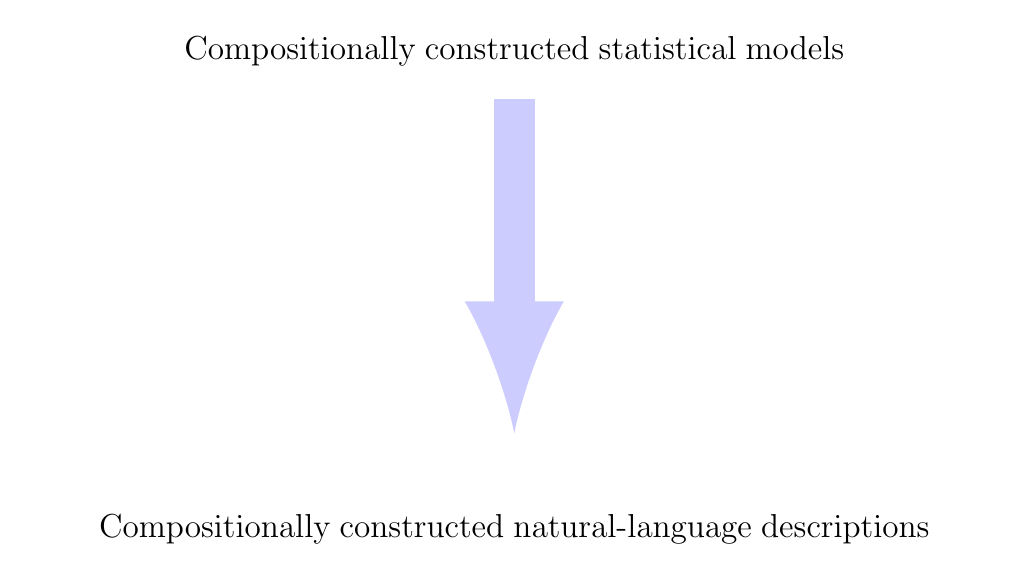
\begin{tikzpicture}
      \node (top_text) [text width=\textwidth, align=center] at (0, 0) {\large Compositionally constructed statistical models};
      \draw [->, >=latex, blue!20!white, line width=15pt] (0, -0.05\textwidth) to (0, -0.4\textwidth);
      \node (bottom_text) [text width=\textwidth, align=center] at (0, -0.5\textwidth) 
      {\large Compositionally constructed natural-language descriptions};
    \end{tikzpicture}
  \end{center}
\end{frame}

\begin{frame}{Defining a language of models}
  \input{figures/flow_chart_language}
\end{frame}

\begin{frame}{A language of Gaussian processes}
  \begin{itemize}
    \item Define probability distributions on functions
    \item Used to perform Bayesian (nonlinear) regression
  \end{itemize}
  \vspace{\baselineskip}
  \begin{center}
    \includegraphics<1>[width=0.8\textwidth]{figures/lin_reg/sq_exp_prior}
    \includegraphics<2>[width=0.8\textwidth]{figures/quad/sq_exp_1}
    \includegraphics<3>[width=0.8\textwidth]{figures/quad/sq_exp_2}
    \includegraphics<4>[width=0.8\textwidth]{figures/quad/sq_exp_3}
    \includegraphics<5>[width=0.8\textwidth]{figures/quad/sq_exp_5}
    \includegraphics<6>[width=0.8\textwidth]{figures/quad/sq_exp_10}
    \includegraphics<7>[width=0.8\textwidth]{figures/quad/sq_exp_15}
  \end{center}
\end{frame}

\begin{frame}{The atoms of our language}  
  \newcommand{\fhbig}{1.0cm}
\newcommand{\fwbig}{1.2cm}
\newcommand{\kernpic}[1]{\includegraphics[height=\fhbig,width=\fwbig]{figures/structure_examples/#1}}
\newcommand{\colsize}{1.7cm}
\newcommand{\sepsize}{0.0cm}

Five base kernels

\vspace{\baselineskip}

\begin{tabularx}{\columnwidth}{x{\colsize}x{\colsize}x{\colsize}x{\colsize}x{\colsize}}
  \kernpic{se_kernel} & \kernpic{per_kernel} & \kernpic{lin_kernel} & \kernpic{c_kernel} & \kernpic{wn_kernel} \\
  {\footnotesize Squared \newline exp. (\kSE)} & {\footnotesize Periodic (\kPer)} & {\footnotesize Linear (\kLin)} & {\footnotesize Constant (\kC)} & {\footnotesize White \newline noise (\kWN)}
\end{tabularx}

\vspace{\baselineskip}

Encoding for the following types of functions

\vspace{\baselineskip}

\begin{tabularx}{\columnwidth}{x{\colsize}x{\colsize}x{\colsize}x{\colsize}x{\colsize}}
  \kernpic{se_kernel_draws} & \kernpic{per_kernel_draws_s2} & \kernpic{lin_kernel_draws} & \kernpic{c_kernel_draws} & \kernpic{wn_kernel_draws} \\
  {\footnotesize Smooth \newline functions} & {\footnotesize Periodic functions} & {\footnotesize Linear \newline functions} & {\footnotesize Constant \newline functions} & {\footnotesize Gaussian \newline noise} 
\end{tabularx}


\end{frame}

\begin{frame}{The composition rules of our language}
\begin{itemize} 
	\item Two main operations: addition, multiplication
\end{itemize}
\newcommand{\fhbig}{1.6cm}
\newcommand{\fwbig}{1.8cm}
\newcommand{\kernpic}[1]{\includegraphics[height=\fhbig,width=\fwbig]{figures/structure_examples/#1}}
\newcommand{\largeplus}{\tabbox{{\Large+}}}
\newcommand{\largeeq}{\tabbox{{\Large=}}}
\newcommand{\largetimes}{\tabbox{{\Large$\times$}}}
\begin{figure}[ht]
\centering
\renewcommand{\tabularxcolumn}[1]{>{\arraybackslash}m{#1}}
\begin{tabularx}{\columnwidth}{XXcXX}
  \kernpic{lin_times_lin} & \kernpic{lin_times_lin_draws} & \phantom{mm}
& \kernpic{longse_times_per} & \kernpic{longse_times_per_draws_s1}
\\
  {\small $\kLin \times \kLin$} & {\small quadratic functions} & \phantom{mm}
& {\small $\kSE \times \kPer$} & {\small locally \newline periodic}
\\ \\
%\midrule 
  \kernpic{lin_plus_per} & \kernpic{lin_plus_per_draws} & \phantom{mm} 
& \kernpic{se_plus_per} & \kernpic{se_plus_per_draws_s7}
\\
  {\small $\kLin + \kPer$} & {\small periodic plus linear trend} & \phantom{mm}
& {\small $\kSE + \kPer$ } & {\small periodic plus smooth trend}
\end{tabularx}
\end{figure}


\end{frame}

\begin{frame}{Automatic translation of models}
  \input{figures/flow_chart_trans}
\end{frame}

\begin{frame}{Sums of kernels are sums of functions}
  If ${\textcolor{red}{f_1} \,\sim\, \gp{}(0, \textcolor{red}{\kernel_1})}$ and independently ${\textcolor{blue}{f_2} \,\sim\, \gp{}(0, \textcolor{blue}{\kernel_2})}$ then
  \begin{align*}
  \textcolor{red}{f_1} + \textcolor{blue}{f_2} \,\sim\, \gp{}(0, \textcolor{red}{\kernel_1} + \textcolor{blue}{\kernel_2})
  \end{align*}
  
\eg

\vspace{\baselineskip}

\begin{tabular}{ccccccc}
\includegraphics[trim=30 0 62 25, clip, width=0.15\textwidth]{figures/03-mauna2003_all} &
\raisebox{0.4cm}{$=$} &
\includegraphics[trim=30 0 62 25, clip, width=0.15\textwidth]{figures/03-mauna2003_1} &
\raisebox{0.4cm}{$+$} &
\includegraphics[trim=30 0 62 25, clip, width=0.15\textwidth]{figures/03-mauna2003_2} &
\raisebox{0.4cm}{$+$} &
\includegraphics[trim=30 0 62 25, clip, width=0.15\textwidth]{figures/03-mauna2003_3}
\end{tabular}

\vspace{\baselineskip}

\begin{tabular}{ccccccc}
\includegraphics[trim=30 0 62 25, clip, width=0.15\textwidth]{figures/01-airline_all} &
\raisebox{0.4cm}{$=$} &
\includegraphics[trim=30 0 62 25, clip, width=0.15\textwidth]{figures/01-airline_1} &
\raisebox{0.4cm}{$+$} &
\includegraphics[trim=30 0 62 25, clip, width=0.15\textwidth]{figures/01-airline_2} &
\raisebox{0.4cm}{$+$} &
\includegraphics[trim=30 0 62 25, clip, width=0.15\textwidth]{figures/01-airline_3}
\end{tabular}

\vspace{\baselineskip}

We can therefore describe each component separately

\end{frame}

\begin{frame}{Products of kernels}
  \begin{align*}
    \phantom{\underbrace{\kSE}_{\textnormal{\scriptsize approximately}} \times }
    \underbrace{\kPer}_{\textnormal{\scriptsize periodic function}} \phantom{\times 
    \underbrace{\kLin}_{\textnormal{\scriptsize with linearly growing amplitude}} \times 
    \underbrace{\boldsymbol{\sigma}}_{\textnormal{\scriptsize until 1700}}}
  \end{align*}
  
  \vspace{\baselineskip}
  
  \begin{itemize}
  	\item Properties of individual kernels well understood
	\item Can be described with standard noun phrase
  \end{itemize}
  
  \vspace{\baselineskip}
  
  \begin{block}{}
    \begin{tabular}{cccc}
      \includegraphics[width=0.2\textwidth]{figures/trans_samples/draw_11} &
      \includegraphics[width=0.2\textwidth]{figures/trans_samples/draw_12} &
      \includegraphics[width=0.2\textwidth]{figures/trans_samples/draw_13} &
      \includegraphics[width=0.2\textwidth]{figures/trans_samples/draw_14}
    \end{tabular}
  \end{block}
\end{frame}

\begin{frame}{Products of kernels}
  \begin{align*}
    \underbrace{\kSE}_{\textnormal{\scriptsize approximately}} \times
    \underbrace{\kPer}_{\textnormal{\scriptsize periodic function}} \phantom{\times 
    \underbrace{\kLin}_{\textnormal{\scriptsize with linearly growing amplitude}} \times 
    \underbrace{\boldsymbol{\sigma}}_{\textnormal{\scriptsize until 1700}}}
  \end{align*}
  
  \vspace{\baselineskip}
  
  \begin{itemize}
  	\item Multiplying by each kernel has a consistent effect
	\item Can be described with consistent adjectives / modifiers
  \end{itemize}
  
  \vspace{\baselineskip}
  
  \begin{block}{}
    \begin{tabular}{cccc}
      \includegraphics[width=0.2\textwidth]{figures/trans_samples/draw_21} &
      \includegraphics[width=0.2\textwidth]{figures/trans_samples/draw_22} &
      \includegraphics[width=0.2\textwidth]{figures/trans_samples/draw_23} &
      \includegraphics[width=0.2\textwidth]{figures/trans_samples/draw_24}
    \end{tabular}
  \end{block}
\end{frame}

\begin{frame}{Products of kernels}
  \begin{align*}
    \underbrace{\kSE}_{\textnormal{\scriptsize approximately}} \times
    \underbrace{\kPer}_{\textnormal{\scriptsize periodic function}} \times 
    \underbrace{\kLin}_{\textnormal{\scriptsize with linearly growing amplitude}} \phantom{\times 
    \underbrace{\boldsymbol{\sigma}}_{\textnormal{\scriptsize until 1700}}}
  \end{align*}
  
  \vspace{\baselineskip}
  
  \begin{itemize}
  	\item Multiplying by each kernel has a consistent effect
	\item Can be described with consistent adjectives / modifiers
  \end{itemize}
  
  \vspace{\baselineskip}
  
  \begin{block}{}
    \begin{tabular}{cccc}
      \includegraphics[width=0.2\textwidth]{figures/trans_samples/draw_31} &
      \includegraphics[width=0.2\textwidth]{figures/trans_samples/draw_32} &
      \includegraphics[width=0.2\textwidth]{figures/trans_samples/draw_33} &
      \includegraphics[width=0.2\textwidth]{figures/trans_samples/draw_34}
    \end{tabular}
  \end{block}
\end{frame}

\begin{frame}{Products of kernels}
  \begin{align*}
    \underbrace{\kSE}_{\textnormal{\scriptsize approximately}} \times
    \underbrace{\kPer}_{\textnormal{\scriptsize periodic function}} \times 
    \underbrace{\kLin}_{\textnormal{\scriptsize with linearly growing amplitude}} \times 
    \underbrace{\boldsymbol{\sigma}}_{\textnormal{\scriptsize until 1700}}
  \end{align*}
  
  \vspace{\baselineskip}
  
  \begin{itemize}
  	\item Multiplying by each kernel has a consistent effect
	\item Can be described with consistent adjectives / modifiers
  \end{itemize}
  
  \vspace{\baselineskip}
  
  \begin{block}{}
    \begin{tabular}{cccc}
      \includegraphics[width=0.2\textwidth]{figures/trans_samples/draw_41} &
      \includegraphics[width=0.2\textwidth]{figures/trans_samples/draw_42} &
      \includegraphics[width=0.2\textwidth]{figures/trans_samples/draw_43} &
      \includegraphics[width=0.2\textwidth]{figures/trans_samples/draw_44}
    \end{tabular}
  \end{block}
\end{frame}

\begin{frame}{Automatically generated reports}
  \input{figures/flow_chart_report}
\end{frame}

\begin{frame}{Example: Solar irradiance}
\newcommand{\wmgd}{0.5\columnwidth}
\newcommand{\hmgd}{3.0cm}
\newcommand{\mdrd}{figures/02-solar}
\newcommand{\mbm}{\hspace{-0.3cm}}
{\footnotesize
\input{\mdrd/02-solar_1_description.tex}
}

\vspace{\baselineskip}

\begin{tabular}{cc}
\mbm \includegraphics[width=\wmgd,height=\hmgd]{\mdrd/02-solar_1} & \includegraphics[width=\wmgd,height=\hmgd]{\mdrd/02-solar_1_cum}
\end{tabular}
\end{frame}

\begin{frame}{Example: Solar irradiance}
\newcommand{\wmgd}{0.5\columnwidth}
\newcommand{\hmgd}{3.0cm}
\newcommand{\mdrd}{figures/02-solar}
\newcommand{\mbm}{\hspace{-0.3cm}}
{\footnotesize
This component is constant.
This component applies from 1644 until 1713.
}

\vspace{\baselineskip}

\begin{tabular}{cc}
\mbm \includegraphics[width=\wmgd,height=\hmgd]{\mdrd/02-solar_2} & \includegraphics[width=\wmgd,height=\hmgd]{\mdrd/02-solar_2_cum}
\end{tabular}
\end{frame}

\begin{frame}{Example: Solar irradiance}
\newcommand{\wmgd}{0.5\columnwidth}
\newcommand{\hmgd}{3.0cm}
\newcommand{\mdrd}{figures/02-solar}
\newcommand{\mbm}{\hspace{-0.3cm}}
{\footnotesize
This component is a smooth function with a typical lengthscale of 21.9 years.
This component applies until 1644 and from 1719 onwards.
}

\vspace{\baselineskip}

\begin{tabular}{cc}
\mbm \includegraphics[width=\wmgd,height=\hmgd]{\mdrd/02-solar_3} & \includegraphics[width=\wmgd,height=\hmgd]{\mdrd/02-solar_3_cum}
\end{tabular}
\end{frame}

\begin{frame}{Example: Solar irradiance}
\newcommand{\wmgd}{0.5\columnwidth}
\newcommand{\hmgd}{3.0cm}
\newcommand{\mdrd}{figures/02-solar}
\newcommand{\mbm}{\hspace{-0.3cm}}
{\footnotesize
This component is approximately periodic with a period of 10.8 years.
Across periods the shape of this function varies smoothly with a typical lengthscale of 36.9 years.
The shape of this function within each period is very smooth and resembles a sinusoid.
This component applies until 1643 and from 1716 onwards.
}

\vspace{\baselineskip}

\begin{tabular}{cc}
\mbm \includegraphics[width=\wmgd,height=\hmgd]{\mdrd/02-solar_4} & \includegraphics[width=\wmgd,height=\hmgd]{\mdrd/02-solar_4_cum}
\end{tabular}
\end{frame}

\begin{frame}{Visit our website - try our (simpler) demo}
  \begin{center}
    \Huge www.automaticstatistician.com
  \end{center}
\end{frame}

\begin{frame}{Appendix}
\end{frame}

\begin{frame}{Goals of the automatic statistician project}
  \begin{itemize}
    \item Provide a set of tools for understanding data that require minimal expert input
    \vspace{\baselineskip}
    \item Uncover challenging research problems in \eg
    \begin{itemize}
      \item Automated inference
      \item Model construction and comparison
      \item Data visualisation and interpretation
      \item Automatic model checking / criticism
    \end{itemize}
    \vspace{\baselineskip}
    \item Make science go faster\dots
    \begin{itemize}
      \item \dots and make it more fun
    \end{itemize}
  \end{itemize}
\end{frame}

\begin{frame}{The kernel determines generalisation}
  \begin{center}
    \only<1>{Long lengthscale SE}
    \only<2>{Short lengthscale SE}
    \only<3>{Long lengthscale SE + Short lengthscale SE}
    \only<4>{SE + SE + SE + SE $\times$ Periodic}
  \end{center}
  \begin{center}
    \includegraphics<1>[width=0.8\textwidth]{figures/mauna-plots/SE-long.pdf}
    \includegraphics<2>[width=0.8\textwidth]{figures/mauna-plots/SE-short.pdf}
    \includegraphics<3>[width=0.8\textwidth]{figures/mauna-plots/SE-SE.pdf}
    \includegraphics<4>[width=0.8\textwidth]{figures/mauna-plots/Complex.pdf}
  \end{center}
\end{frame}

\begin{frame}{Modeling changepoints}
We can model transitions between regimes : let $\textcolor{red}{f_1(x)} \sim \gp{}(0,k_1)$ and $\textcolor{blue}{f_2(x)} \sim \gp{}(0,k_2)$ and then define
\[
f(x) = (1-\sigma(x))\, \textcolor{red}{f_1(x)} + \sigma(x)\, \textcolor{blue}{f_2(x)}
\]

where $\sigma$ is a sigmoid function between 0 and 1.

\vspace{2\baselineskip}

Then $f \sim \gp{}(0,k)$, where
\[
k(x,x') = (1-\sigma(x)) \, \textcolor{red}{k_1(x,x')}  \, (1-\sigma(x')) + \sigma(x) \,
\textcolor{blue}{k_2(x,x')} \, \sigma(x') 
\]

We define the changepoint operator $\kernel = \kCP(\kernel_1, \kernel_2)$.

\end{frame}

\begin{frame}{An expressive language of models}
\begin{center}
\begin{tabular}{l|l}
Regression model & Kernel \\
\midrule
\gp{} smoothing & $\kSE + \kWN$ \\
Linear regression & $\kC + \kLin + \kWN$ \\
Multiple kernel learning & $\sum \kSE$ + \kWN\\
Trend, cyclical, irregular & $\sum \kSE + \sum \kPer$ + \kWN\\
Fourier decomposition & $\kC + \sum \cos$ + \kWN\\
Sparse spectrum \gp{}s & $\sum \cos$ + \kWN\\
Spectral mixture & $\sum \SE \times \cos$ + \kWN\\
Changepoints & \eg $\kCP(\kSE, \kSE) + \kWN$ \\
Heteroscedasticity & \eg $\kSE + \kLin \times \kWN$
\end{tabular}
\end{center}
Note: $\cos$ is a special case of our version of $\kPer$
\end{frame}

\begin{frame}{Example: Mauna Loa Keeling Curve}
\hspace{-1.2cm}
\only<1>{\includegraphics[width=0.4\textwidth]{figures/11-Feb-v4-03-mauna2003-s_max_level_0/03-mauna2003-s_all_small.pdf}}
\only<2>{\includegraphics[width=0.4\textwidth]{figures/11-Feb-v4-03-mauna2003-s_max_level_1/03-mauna2003-s_all_small.pdf}}
\only<3>{\includegraphics[width=0.4\textwidth]{figures/11-Feb-v4-03-mauna2003-s_max_level_2/03-mauna2003-s_all_small.pdf}}
\only<4>{\includegraphics[width=0.4\textwidth]{figures/11-Feb-v4-03-mauna2003-s_max_level_3/03-mauna2003-s_all_small.pdf}}

\vspace{-3.5cm}
\begin{minipage}[t][14cm][t]{1.14\linewidth}
\begin{flushleft}
\hspace{5.5cm}
\vspace{-8cm}
\makebox[\textwidth][c]{
\raisebox{10cm}{
\vspace{-8cm}
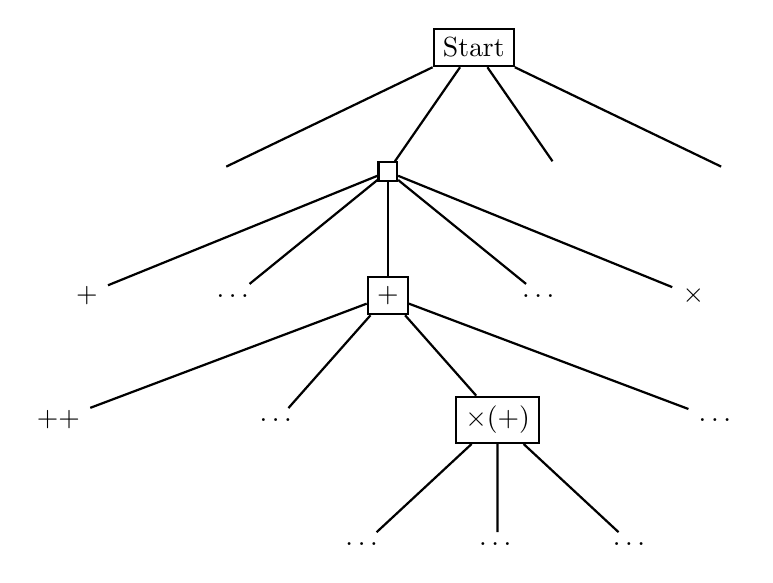
\begin{tikzpicture}
[sibling distance=0.18\columnwidth,-,thick, level distance=0.13\columnwidth]
%\footnotesize
\node[shape=rectangle,draw,thick] {Start}
%\pause
  child {node {$\SE$}}
%  fill=camlightblue!30
  child {node[shape=rectangle,draw,thick] {$\RQ$}
    [sibling distance=0.16\columnwidth]
%    {\visible<2->{ child {node {\ldots}}}}
    child [hide on=-1] {node {$\SE$ + \RQ}}
    child [hide on=-1] {node {\ldots}}
    child [hide on=-1] {node[shape=rectangle,draw,thick] {$\Per + \RQ$}
      [sibling distance=0.23\columnwidth]
      child [hide on=-2] {node {$\SE + \Per + \RQ$}}
      child [hide on=-2] {node {\ldots}}
      child [hide on=-2] {node[shape=rectangle,draw,thick] {$\SE \times (\Per + \RQ)$}
        [sibling distance=0.14\columnwidth]
        child [hide on=-3] {node {\ldots}}
        child [hide on=-3] {node {\ldots}}
        child [hide on=-3] {node {\ldots}}
      }
      child [hide on=-2] {node {\ldots}}
    }
    %child {node {$\RQ \times \SE$}}
    child [hide on=-1] {node {\ldots}}
    child [hide on=-1] {node {$\Per \times \RQ$}}
  }
  child {node {$\Lin$}}
  child {node {$\Per$}}
  ;
\end{tikzpicture}}
}\end{flushleft}
\end{minipage}
\only<4>{}
\end{frame}\begin{frame}{Products of kernels - $\kSE$}
  \begin{align*}
    \underbrace{\kSE}_{\textnormal{\scriptsize approximately}} \times
    \underbrace{\kPer}_{\textnormal{\scriptsize periodic function}} \phantom{\times 
    \underbrace{\kLin}_{\textnormal{\scriptsize with linearly growing amplitude}} \times 
    \underbrace{\boldsymbol{\sigma}}_{\textnormal{\scriptsize until 1700}}}
  \end{align*}
  
  \vspace{\baselineskip}
  
  {\bf Multiplication by $\kSE$} removes long range correlations from a model since $\kSE(x,x')$ decreases monotonically to 0 as $|x - x'|$ increases.
  
  \vspace{\baselineskip}
  
  \begin{block}{}
    \begin{tabular}{cccc}
      \includegraphics[width=0.2\textwidth]{figures/trans_samples/draw_21} &
      \includegraphics[width=0.2\textwidth]{figures/trans_samples/draw_22} &
      \includegraphics[width=0.2\textwidth]{figures/trans_samples/draw_23} &
      \includegraphics[width=0.2\textwidth]{figures/trans_samples/draw_24}
    \end{tabular}
  \end{block}
\end{frame}

\begin{frame}{Products of kernels - $\kLin$}
  \begin{align*}
    \underbrace{\kSE}_{\textnormal{\scriptsize approximately}} \times
    \underbrace{\kPer}_{\textnormal{\scriptsize periodic function}} \times 
    \underbrace{\kLin}_{\textnormal{\scriptsize with linearly growing amplitude}} \phantom{\times 
    \underbrace{\boldsymbol{\sigma}}_{\textnormal{\scriptsize until 1700}}}
  \end{align*}
  
  \vspace{\baselineskip}
  
  {\bf Multiplication by $\kLin$} is equivalent to multiplying the function being modeled by a linear function.
If $f(x) \,\sim\, \gp{}(0, \kernel)$, then $x\,f(x) \,\sim\, \gp{}\left(0, k \times \kLin \right)$.
This causes the standard deviation of the model to vary linearly without affecting the correlation.
  
  \vspace{\baselineskip}
  
  \begin{block}{}
    \begin{tabular}{cccc}
      \includegraphics[width=0.2\textwidth]{figures/trans_samples/draw_31} &
      \includegraphics[width=0.2\textwidth]{figures/trans_samples/draw_32} &
      \includegraphics[width=0.2\textwidth]{figures/trans_samples/draw_33} &
      \includegraphics[width=0.2\textwidth]{figures/trans_samples/draw_34}
    \end{tabular}
  \end{block}
\end{frame}

\begin{frame}{Products of kernels - changepoints}
  \begin{align*}
    \underbrace{\kSE}_{\textnormal{\scriptsize approximately}} \times
    \underbrace{\kPer}_{\textnormal{\scriptsize periodic function}} \times 
    \underbrace{\kLin}_{\textnormal{\scriptsize with linearly growing amplitude}} \times 
    \underbrace{\boldsymbol{\sigma}}_{\textnormal{\scriptsize until 1700}}
  \end{align*}
  
  \vspace{\baselineskip}
  
  {\bf Multiplication by $\boldsymbol\sigma$} is equivalent to multiplying the function being modeled by a sigmoid.
  
  \vspace{\baselineskip}
  
  \begin{block}{}
    \begin{tabular}{cccc}
      \includegraphics[width=0.2\textwidth]{figures/trans_samples/draw_41} &
      \includegraphics[width=0.2\textwidth]{figures/trans_samples/draw_42} &
      \includegraphics[width=0.2\textwidth]{figures/trans_samples/draw_43} &
      \includegraphics[width=0.2\textwidth]{figures/trans_samples/draw_44}
    \end{tabular}
  \end{block}
\end{frame}

\begin{frame}{Noun phrase and postmodifier forms}
  \begin{center}
    \footnotesize
    \begin{tabular}{l|l|l}
      Kernel & Noun phrase & Postmodifier phrase \\
      \midrule
      $\kWN$  & uncorrelated noise & n/a\\
      $\kC$   & constant & n/a \\
      $\kSE$  & smooth function & whose shape changes smoothly\\
      $\kPer$ & periodic function & modulated by a periodic function\\
      $\kLin$ & linear function & with linearly varying amplitude\\ 
      $\prod_k \kLin^{(k)}$ & polynomial & with polynomially varying amplitude\\
      $\prod_k \boldsymbol{\sigma}^{(k)}$ & n/a & which applies until / from [changepoint]
    \end{tabular}
  \end{center}
\end{frame}

\begin{frame}{Challenges}
  \begin{itemize}
    \item Computational complexity of searching through a huge space of models
    \vspace{\baselineskip}
    \item Increasing the expressivity of language
    \begin{itemize}
      \item \eg Monotonocity, positive functions, symmetries
    \end{itemize}
    \vspace{\baselineskip}
    \item Interpretability / accuracy
    \vspace{\baselineskip}
    \item Extending the automatic reports to multidimensional datasets
    \begin{itemize}
      \item Search and descriptions naturally extend to multiple dimensions, but automatically generating relevant visual summaries harder 
    \end{itemize}
  \end{itemize}
\end{frame}

\begin{frame}{Current and future directions}
  \begin{itemize}
    \item Multivariate linear regression
    \vspace{\baselineskip}
    \item Multivariate non-linear regression
    \vspace{\baselineskip}
    \item Classification, point processes, \dots
    \vspace{\baselineskip}
    \item Completing and interpreting tables and databases
    \vspace{\baselineskip}
  \end{itemize}
\end{frame}

\end{document}

\begin{frame}{Title}
  \begin{itemize}
    \item Content
    \vspace{\baselineskip}
    \item Content
    \vspace{\baselineskip}
    \item Content
    \begin{itemize}
       \item Content
       \item Content
     \end{itemize}
  \end{itemize}
\end{frame}